\section{Selection procedure}
\label{sec:procedure}

\subsection{Inputs}
\label{sec:procedure-inputs}

A candidate population of datasheet records; room volume, distance and
leakage model; $f_1$, $f_{\mathrm{sp}}$, $f_2$, target levels and channel
layout; the per-driver amplifier limits; preferred $\Qtc^\ast$ and
per-driver box-volume cap; allowed diameter and unit-count ranges; any
manifold crossover ceiling; the hard $\Xmax$ boundary with preferred
excursion margin; the Doppler sideband-ratio budget; mono-bass stereo
summing credit; and the declared transient waveform family. All are fields
of one serializable scenario or study definition. The canonical values of
\cref{sec:scope-scenario} merely instantiate those inputs.

\subsection{Algorithm}
\label{sec:procedure-algorithm}

\begin{enumerate}
\item \textbf{Normalize and quality-check} each record: required fields
	present, $\Xmax$ and $\Pmax$ conventions recorded, derived quantities
	(for example $\Bl$ from $F_s,\Qes,\Mms,\Re$) flagged as derived, records
	with missing required fields skipped and counted.
\item \textbf{Compute descriptors}: $\Vd$, $\eta_0\Pmax$ \cref{eq:eta0},
	the corner rate $F_s/\Qts$ \cref{eq:cornerrate}, $f_L$, and the regime
	boundary $f_x$ \cref{eq:fx}.
\item \textbf{Select a physical alignment}: target the role's corner
	($f_{\mathrm{pz}}$ for low bass, $f_{\mathrm{sp}}$ for upper bass) under
	\cref{eq:Fsrule} and the preferred $\Qtc^\ast$. If that box is
	nonphysical or exceeds the per-driver volume cap, use the cap and retain
	the resulting $\Qtc$ and $F_c$. Alignment mismatch is recorded, not
	rejected.
\item \textbf{Evaluate room demand} \cref{eq:Vdem} across the complete role
	band, dividing by physical units under A9. For a full-band stereo
	channel, use the low-bass target minus the declared summing credit below
	$f_{\mathrm{sp}}$ and the independent-channel target above it.
\item \textbf{Evaluate steady requirements} \cref{eq:Ereq,eq:Ireq,eq:Preq}
	and \textbf{transient requirements} \cref{eq:ctr} over the band and the
	declared start phases, retaining the worst value and the frequency at
	which it occurs.
\item \textbf{Apply the hard gates} of \cref{sec:risk-policy}, recording
	the binding gate for every rejected candidate.
\item \textbf{Report the risk vector} \cref{eq:riskvec} for every surviving
	candidate.
\item \textbf{Assign Pareto fronts} on the role's core objectives.
\item \textbf{Apply the declared lexicographic order} within each front to
	obtain a reproducible total order.
\item \textbf{Scale repeated identical units}: displacement, voltage,
	current and Doppler indicators scale as $1/N$, electrical power as
	$1/N^2$, and total enclosure volume as $N\Vb$. The individual driver
	alignment is unchanged because the box cap is per unit.
\item \textbf{Assemble architectures}: form split-role systems without
	summing unlike role indicators, and full-band stereo systems from one
	model and count per channel. Reject a split whose nominal crossover
	exceeds the declared manifold ceiling.
\item \textbf{Compare complete systems} by Pareto fronts in steady and
	transient excursion, Doppler ratio, amplifier utilization, total
	enclosure volume, and physical driver count. No weighted architecture
	score is formed.
\item \textbf{Re-run} the ranking under the declared uncertainty, summing
	and policy variants (\cref{sec:procedure-robustness}), flagging
	candidates whose position is unstable.
\end{enumerate}

Every candidate ends in exactly one of four statuses: \emph{rejected} (with
the binding gate), \emph{feasible but dominated}, \emph{Pareto-optimal}, or
\emph{recommended by policy} (first in its role's order). Only the last is
a recommendation; the first three are reported so a reader with different
priorities can re-rank without re-deriving anything.

\subsection{Candidate population and the private-data boundary}
\label{sec:procedure-database}

The candidate population used for the aggregate evidence in this report is
a locally held export of a community driver database. That file is obtained
separately and is not redistributed. What is published is its SHA-256 hash,
the parser and filter definitions, the retained and skipped record counts,
role-feasible and Pareto-front counts, and the aggregate plots of
\cref{fig:database-pareto}. Those quantities are collected in
\cref{tab:database-summary}, which is generated directly from the frozen
input and is the authoritative source for every count referred to in the
text. The driver records used in \cref{app:example} come from the
manufacturers' public datasheets and are reproduced in full, so the worked
example is reproducible without access to the private file.

\begin{figure}[htbp]
	\centering
	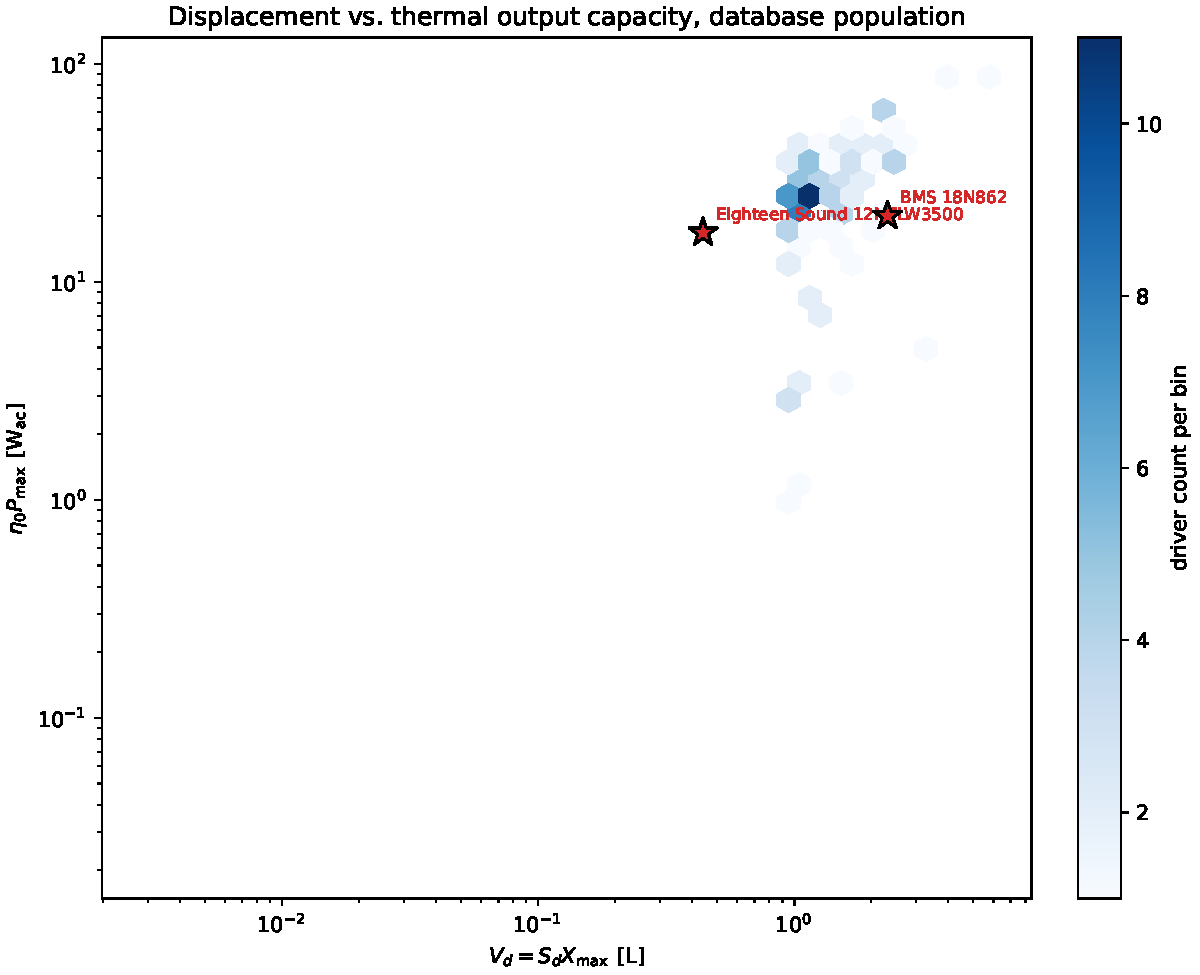
\includegraphics[width=\columnwidth]{../figures/fig_database_pareto}
	\caption{Frozen candidate population in the $(\Vd,\eta_0\Pmax)$ plane,
	shown as a binned density so that no individual record is disclosed. The
	two candidates selected in \cref{app:example} are marked. Aggregate
	population evidence only; the counts behind it are in
	\cref{tab:database-summary}.}
	\label{fig:database-pareto}
\end{figure}

\begin{table*}[htbp]
\centering
\caption{Private driver-database evidence summary at the worked unit counts (aggregate counts only. The accompanying manifest supplies the full source hash, parser, and filter definitions).}
\label{tab:database-summary}
\begin{tabular}{lr}
\toprule
quantity & value\\
\midrule
source hash (SHA-256, first 12 hex) & \texttt{0a5edbd1868e}\\
retained rows & 1342\\
skipped rows (missing required fields) & 537\\
sub-manifold role candidates (15--21in) & 246\\
sub-manifold role feasible (2 total) & 1\\
sub-manifold role Pareto front & 1\\
upper-bass role candidates (8--15in) & 592\\
upper-bass role feasible (1/channel) & 146\\
upper-bass role Pareto front & 41\\
both role tests feasible at worked counts (size-unrestricted) & 1\\
\bottomrule
\end{tabular}
\end{table*}


The observation this evidence supports is deliberately narrow: in this
frozen population, under this scenario, the candidates selected for the two
roles occupy different regions of the $(\Vd,\eta_0\Pmax)$ plane, differing
chiefly in displacement volume at comparable thermal output capacity.
Overlap between driver-level role populations does not establish that one
stereo full-band system meets both channel reference bases within the
allowed sizes and counts; that system question is evaluated next.

\subsection{Crossover and architecture sensitivity}
\label{sec:procedure-architecture}

The crossover is swept in \SI{5}{\hertz} increments before selecting the
worked system. For the public Dayton/Faital pair of
\cref{app:example}, \SI{60}{\hertz} fails upper-driver excursion and
Doppler gates, \SI{65}{\hertz} remains Doppler-limited, and
\SIrange{70}{80}{\hertz} is feasible. The upper role continues to gain
margin above \SI{80}{\hertz}, but those points are driver-only
counterfactuals because the illustrative manifold declares
\SI{80}{\hertz} as its highest nominal crossover. The implemented
low-pass must still suppress manifold output above its validated acoustic
band.

\begin{figure}[htbp]
	\centering
	\includegraphics[width=\columnwidth]{../figures/fig_split_sensitivity}
	\caption{Worked-pair crossover sensitivity. Hard-feasible points at or
	below the declared manifold ceiling are distinguished from rejected
	points and driver-only counterfactuals above the ceiling. The selected
	\SI{80}{\hertz} point maximizes upper-driver margin only within the
	declared feasible interval; it is not a universal optimum.}
	\label{fig:split-sensitivity}
\end{figure}

\begin{table*}[htbp]
\centering
\caption{Crossover sensitivity with every other scenario input fixed. Candidate entries are hard-feasible/preferred-margin record counts in the declared role pools. The public worked pair is re-aligned and its enclosure recalculated at every crossover. Points above the declared manifold ceiling are driver-only counterfactuals (CF), not valid manifold recommendations. $F/P$ denotes hard-feasible/preferred-margin records.}
\label{tab:split-sensitivity}
\scriptsize
\setlength{\tabcolsep}{2pt}
\begin{tabular}{rrrrrrrl}
\toprule
$f_{\mathrm{sp}}$ [Hz] & valid & sub $F/P$ & upper $F/P$ & worked $\xi_s/\xi_u$ & $V_{b,u}$ [L] & $d_{\mathrm D,u}$ & status\\
\midrule
60 & yes & 1/1 & 62/21 & 0.80/1.09 & 46.2 & 0.025 & reject\\
65 & yes & 1/1 & 89/44 & 0.80/0.91 & 33.0 & 0.021 & reject\\
70 & yes & 1/1 & 110/76 & 0.80/0.76 & 25.3 & 0.018 & preferred\\
75 & yes & 1/1 & 129/102 & 0.80/0.65 & 20.2 & 0.016 & preferred\\
80 & yes & 1/1 & 146/115 & 0.80/0.56 & 16.6 & 0.014 & preferred\\
85 & no & 1/1 & 171/134 & 0.80/0.50 & 15.7 & 0.012 & preferred; CF\\
90 & no & 1/1 & 183/146 & 0.80/0.46 & 15.7 & 0.011 & preferred; CF\\
95 & no & 1/1 & 199/165 & 0.80/0.43 & 15.7 & 0.010 & preferred; CF\\
100 & no & 1/1 & 216/176 & 0.80/0.40 & 15.7 & 0.009 & preferred; CF\\
105 & no & 1/1 & 234/191 & 0.80/0.38 & 15.7 & 0.008 & preferred; CF\\
110 & no & 1/1 & 244/204 & 0.80/0.36 & 15.7 & 0.007 & preferred; CF\\
115 & no & 1/1 & 250/219 & 0.80/0.34 & 15.7 & 0.007 & preferred; CF\\
120 & no & 1/1 & 257/228 & 0.80/0.32 & 15.7 & 0.006 & preferred; CF\\
\bottomrule
\end{tabular}
\end{table*}


To test whether the two-role result is merely assumed, a factorial study
compares it with the favourable full-band stereo baseline B5. The inputs
span room volumes of 40, 60 and \SI{90}{\cubic\meter}; nominal crossovers
of 60, 80, 100 and \SI{120}{\hertz}; upper edges of 200, 250 and
\SI{350}{\hertz}; and low-bass targets of 105, 110 and \SI{115}{dB}, with
the independent upper target \SI{5}{dB} lower. Packaging searches use
15--21-inch low-bass drivers in even totals of 2, 4 or 6;
8--15-inch upper drivers at one or two per channel; and 10--18-inch
full-band drivers at one or two per channel.

Because unreported voice-coil inductance makes a 200--\SI{350}{\hertz}
role unevaluable, the primary comparison requires reported $\Le$. In the
canonical 60-\si{\cubic\meter}, 80/250-\si{\hertz},
110/105-\si{dB} case, 119 unique low-bass records and 301 upper-bass
records are feasible at one or more allowed counts, whereas no full-band
record is feasible. The split architecture therefore occupies the
data-complete system Pareto frontier alone in that case. If missing
inductance is permitted, one full-band record survives, but its
upper-band validity remains unresolved; reducing the assumed stereo bass
summing credit from 6 to \SI{3}{dB} removes even that survivor.

\begin{figure}[htbp]
	\centering
	\includegraphics[width=\columnwidth]{../figures/fig_architecture_comparison}
	\caption{Outcome of the 108-scenario architecture study. Each scenario
	is evaluated with the same physical and electronics gates and then
	compared on six separate system objectives. Empty or single-architecture
	fronts are reported rather than converted into a success-shaped score.}
	\label{fig:architecture-comparison}
\end{figure}

\begin{table*}[htbp]
\centering
\caption{Architecture comparison over the declared domestic/mastering factorial. Each target has 36 cases: three room/longest-dimension pairs, four crossovers, and three upper-band edges. Upper-bass target is 5 dB below the listed low-bass target. Upper/full candidates must report $L_e$. ``Separate radiators'' compares the two-role architecture at every tested crossover; ``80-Hz manifold'' removes split designs above the declared manifold ceiling. Counts are scenario cases, not combinatorial driver-pair counts.}
\label{tab:architecture-comparison}
\scriptsize
\setlength{\tabcolsep}{3pt}
\begin{tabular}{lrrrrrrr}
\toprule
basis & $L_{\mathrm{sub}}$ [dB] & split feas. & full feas. & split only & mixed & full only & neither\\
\midrule
separate radiators & 105 & 36 & 24 & 12 & 24 & 0 & 0\\
80-Hz manifold & 105 & 18 & 24 & 6 & 12 & 12 & 6\\
separate radiators & 110 & 36 & 16 & 20 & 16 & 0 & 0\\
80-Hz manifold & 110 & 18 & 16 & 10 & 8 & 8 & 10\\
separate radiators & 115 & 36 & 0 & 36 & 0 & 0 & 0\\
80-Hz manifold & 115 & 18 & 0 & 18 & 0 & 0 & 18\\
\bottomrule
\end{tabular}
\end{table*}


Across all tested crossovers, split systems are feasible in all 36 cases at
each target. Full-band systems share the Pareto front in 24 of 36 cases at
\SI{105}{dB} and 16 of 36 at \SI{110}{dB}, but none at
\SI{115}{dB}. Enforcing the illustrative \SI{80}{\hertz} manifold ceiling
removes the split architecture from the 100- and
\SI{120}{\hertz} cases by definition; this creates full-band-only and
neither-feasible outcomes. The two panels therefore separate a
driver/system tradeoff from an external manifold-integration limit.

This supports role specialization for the stated population and envelope,
not a universal motor theorem. Different amplifier, package, room, target
or candidate inputs can restore a full-band frontier member, and the tool
is designed to report it when they do. Current regional price is considered
only after the technical shortlist; the canonical strict case has no
data-complete full-band finalist for a symmetric price comparison.

\subsection{Rank robustness}
\label{sec:procedure-robustness}

Public data is imprecise, and the lexicographic order is a policy. The
ranking is therefore recomputed under declared perturbations---$\Xmax$
scaled by $\pm25\%$, $\Pmax$ shifted by $\pm\SI{3}{dB}$, alternative room
leakage corners, and alternative reasonable lexicographic
orders---and the overlap of the top-$k$ shortlist with the baseline is
reported (\cref{fig:rank-robustness}). If fewer than $k$ baseline records
are feasible, retention is normalized by the records actually available,
not by $k$.

\begin{figure}[htbp]
	\centering
	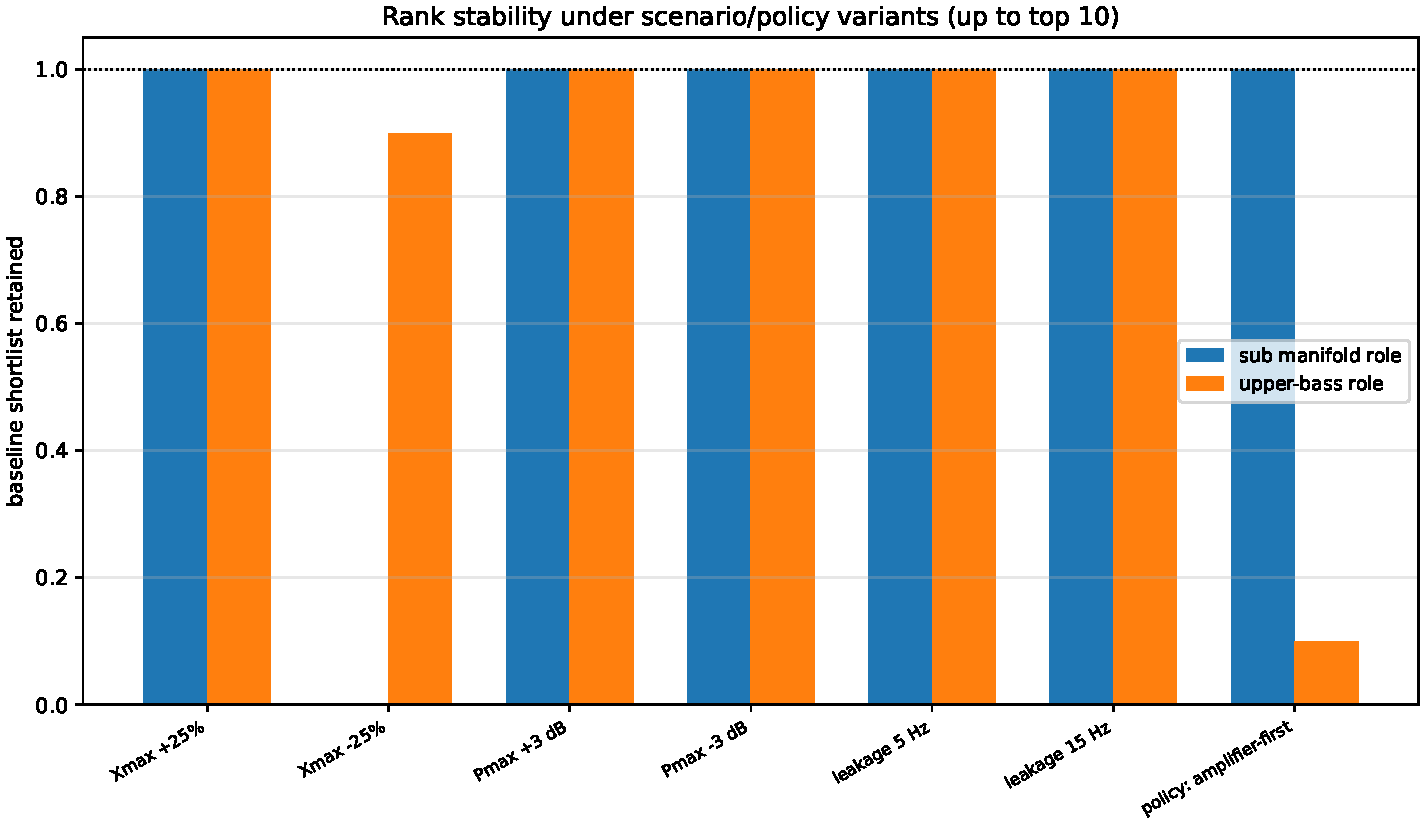
\includegraphics[width=\columnwidth]{../figures/fig_rank_robustness}
	\caption{Top-$k$ shortlist overlap with the baseline ranking under
	declared datasheet, room, and policy perturbations, for both roles. A
	high overlap indicates that the shortlist does not depend on the precise
	value of an uncertain input; a low one identifies where the
	recommendation is provisional.}
	\label{fig:rank-robustness}
\end{figure}

Power-rating and leakage variants retain every baseline record in both
roles. Reducing $\Xmax$ by 25\% removes the sole feasible two-driver
low-bass record and changes one member of the upper top ten. Reordering by
amplifier headroom retains the sole low-bass record but only one of the
upper ten. The low-bass result is therefore binary rather than evidence of
a broad stable shortlist; $\Xmax$ convention and upper-role policy remain
material and are reported with the recommendation.

This is a sensitivity analysis of the decision procedure. It is
\emph{not} physical validation: it does not test the nonlinear indicators
against measured large-signal behaviour. Such validation would require
public $Bl(x)$, $K_{\mathrm{ms}}(x)$, or distortion-headroom measurements
for a comparable subset of candidates, and is identified in
\cref{sec:conclusion} as the principal outstanding item.
